\documentclass[12pt,a4paper,parskip=full]{scrartcl}

\usepackage{bbding}
\usepackage{pifont}
\usepackage{wasysym}
\usepackage[margin=1in]{geometry}
\geometry{letterpaper}
\usepackage{xcolor}
\definecolor{red}{HTML}{cc0000}
\definecolor{gray}{HTML}{666666}
\usepackage{sectsty}
\sectionfont{\color{red}}
\subsectionfont{\color{red}}
\usepackage{graphicx}
\usepackage{hyperref}
\usepackage{amssymb}
\usepackage[style=footnote-dw]{biblatex}
\bibliography{S@SGuideBib}
\setlength\bibitemsep{0.5\baselineskip}

\usepackage{enumitem}
\setitemize{noitemsep}
% \setlist{noitemsep, topsep=-5pt}
% \setlength\itemsep{-0.10em}

\renewcommand{\labelitemi}{$\cdot$}
\renewcommand{\labelitemii}{$\cdot$}
\makeatletter
\let\latexl@section\l@section
\def\l@section#1#2{\begingroup\let\numberline\@gobble\latexl@section{#1}{#2}\endgroup}
\makeatother

\usepackage[T1]{fontenc}
\fontfamily{verdana}

\usepackage{scrlayer-scrpage}{}
\makeatletter
\renewcommand{\@seccntformat}[1]{}
\makeatother

\setlength\parindent{0pt}{}

\title{\Huge{\color{red}\textbf{La Guida a Scrum@Scale
\textsuperscript{\copyright}
}}}
\subtitle{\color{gray}La guida definitiva a Scrum@Scale:\\ Lo scaling che funziona}
% \author{}
\date{}


\begin{document}

%\tableofcontents
%\newpage

\section{Scopo della Guida a Scrum@Scale}
Scrum, come originariamente descritto nella Scrum Guide, è un 
framework per sviluppare, consegnare e mantenere prodotti complessi da 
un singolo team. Fin dalla nascita, il suo uso si è esteso alla creazione di 
prodotti, processi, servizi e sistemi che richiedevano il lavoro di più team.
Scrum@Scale è stato creato per coordinare efficientemente questo nuovo 
ecosistema di team in un modo da ottimizzarsi per perseguire la strategia 
globale dell'organizzazione. Viene raggiunto questo obiettivo creando la 
minima burocrazia possibile grazie ad una architettura ad invarianza di scala 
(scale-free architecture), che estende naturalmente il modo in cui i singoli 
team Scrum funzionano lungo tutta l'organizzazione.

Questa guida contiene la definizione dei componenti che costituiscono Scrum@Scale, includendo le corrispondenti su larga scala dei ruoli, degli eventi e degli artefatti, così come le regole che li tengono insieme.

Il Dr. Jeff Sutherland ha sviluppato Scrum@Scale basandosi sui principi fondamentali di Scrum, della teoria dei sistemi adattivi complessi, la teoria dei giochi e la programmazione ad oggetti. Questa guida è stata sviluppata grazie ai suggerimenti di numerosi praticanti esperti di Scrum e basata sui risultati del loro lavoro. L'obiettivo di questa guida è di rendere il lettore in grado di implementare Scrum@Scale in proprio.

\subsection{Perché Scrum@Scale?}
Scrum è stato disegnato per permettere ad un singolo team di lavorare 
alla sua capacità ottimale mantenendo un ritmo sostenibile. Sul campo è
stato notato che all'aumentare dei team scrum all'interno di una organizzazione,
la capacità ottimale (prodotto funzionante) e la velocity di questi team inizia a
decadere (a causa di problemi come le dipendenze tra team e la duplicazione
del lavoro). Diventa quindi ovvio che serviva un framework per coordinare 
efficacemente questi team in modo da ottenere una scalabilità lineare.
Scrum@Scale è stato ideato per raggiungere questo obiettivo grazie alla
sua architettura a invarianza di scala.

Utilizzando una architettura ad invarianza di scala, l'organizzazione non ha 
vincoli di crescere un particolare modo o secondo un insieme arbitrario di
regole; invece può crescere in maniera organica basandosi sui suoi personali
bisogni e ad un ritmo sostenibile di cambiamento, che possa essere 
accettato dai gruppi di individui che compongono l'organizzazione.

Scrum@Scale è pensato per estendersi lungo tutta l'organizzazione: tutti
i dipartimenti, prodotti e servizi. Può essere applicato lungo diversi domini
in qualsiasi tipo di organizzazione in industrie, governi o accademie.

\subsection{Definizione di Scrum@Scale}
Scrum: Un framework con cui le persone possono risolvere problemi adattivi complessi,
producendo e creando creativamente dei prodotti funzionanti del più alto valore possibile.

La Scrum Guide è l'insieme minimo di regole che permettono ispezione e adattabilità
attraverso una trasparenza radicale per creare innovazione, soddisfazione dei clienti,
performance e felicità del team.

Scrum@Scale: Un framework con cui una rete di team Scrum opera in maniera consistente
alla Scrum Guide per indirizzare problemi adattivi complessi producendo e creando creativamente dei prodotti funzionanti del più alto valore possibile.

\textbf{NOTA:} Questi ``prodotti'' possono essere hardware, software, sistemi complessi integrati, processi, servizi, ecc., a seconda del dominio dei team Scrum.

Scrum@Scale è:
\begin{itemize}
\item Leggero - la minima burocrazia sostenibile
\item Semplice da capire - consiste soltanto di team Scrum
\item Difficile da padroneggiare - richiede di implementare un nuovo modello operativo
\end{itemize}

Scrum@Scale è un framework per scalare Scrum. Semplifica radicalmente lo scaling 
in quanto usa Scrum per scalare Scrum.

In Scrum, è stato separata con cura la responsabilità del ``cosa'' dal ``come''.
La stessa cura è stata mantenuta in Scrum@Scale in modo che la giurisdizione e le responsabilità siano espressamente comprese in modo da eliminare conflitti organizzativi e sprechi che impediscano ai team di raggiungere la loro produttività ottimale.

Scrum@Scale è costituito da componenti che consentono ad un'organizzazione di personalizzare la propria strategia di trasformazione e implementazione. Permette di indirizzare le azioni di cambiamento incrementalmente e dando priorità alle aree che si ritiene più importanti, o più bisognose di cambiamento, e di progredire successivamente nelle altre.

Nel separare queste due giurisdizioni, Scrum@Scale contiene due cicli: il ciclo degli Scrum Master (il ``come'') ed il ciclo dei Product Owner (il ``cosa''), intersecandosi in due punti. Presi insieme, questi cicli producono una potente struttura per coordinare gli sforzi di più team lungo un singolo percorso.

\subsection{I componenti del framework Scrum@Scale\textregistered}

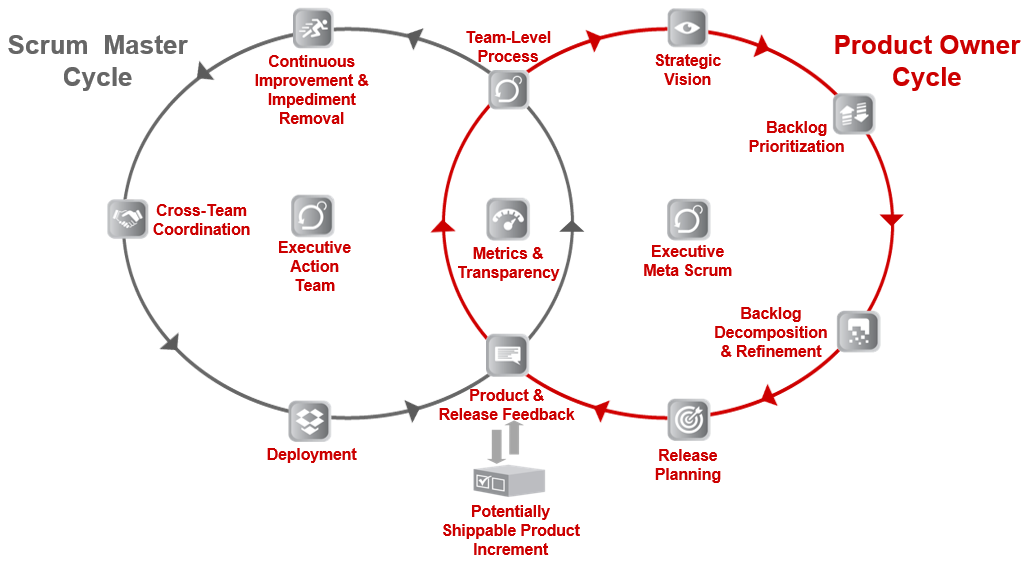
\includegraphics[width=1.0\linewidth]{SMPO-Cycle.png}

\subsection{Cultura guidata dai valori}

Oltre a separare la responsabilità del ``cosa'' e del ``come'' Scrum@Scale si propone inoltre di creare organizzazioni sane creando una cultura basata sui valori in un contesto empirico. I valori di Scrum sono: apertura, coraggio, focus, rispetto e impegno. Questi valori guidano un processo decisionale empirico, che dipende dai tre pilastri di trasparenza, ispezione e adattamento.

L'apertura supporta la trasparenza in tutto il lavoro ed i processi, senza la quale non c'è possibilità di ispezionarli onestamente e tentare di adattarli per il meglio. Il coraggio si riferisce a prendere le difficili decisioni richieste dal fornire valore il più rapidamente possibile ed in maniera innovativa.

Focus e impegno si riferiscono al modo con cui gestiamo i nostri obblighi lavorativi, mettendo come più alta priorità la consegna di valore al cliente. Infine, tutto questo deve avvenire in un ambiente basato sul rispetto per gli individui che svolgono il lavoro, senza il quale nulla può essere creato.

Scrum@Scale aiuta le organizzazioni a prosperare supportando un modello di leadership trasformazionale che promuova un ambiente lavorativo positivo con un ritmo sostenibile e mettendo l'impegno a consegnare valore visibile al cliente come frutto dei nostri sforzi.

\subsection{Come iniziare con Scrum@Scale}
Quando si intende implementare una grande rete di team, è fondamentale sviluppare prima un \textbf{Modello di Riferimento} con un piccolo gruppo di team. Qualsiasi carenza si implementi inizialmente, questa verrà poi amplificata quando si estende il metodo a molteplici team. Molti dei problemi iniziali di estensione del metodo saranno di tipo organizzativi, delle procedure e pratiche di sviluppo che bloccano i team da raggiungere prestazioni elevate e creano frustrazione.

Pertanto, la prima sfida è creare un piccolo gruppo di team che implementino bene lo Scrum. Questo insieme di team permette di risolvere gli impedimenti organizzativi che bloccano l'agilità e creare un modello di riferimento di Scrum che funzioni in quel contesto e che può essere utilizzato come riferimento per l'estensione di Scrum in tutta l'organizzazione.

Via via che il modello di riferimento dei team si estende, gli ostacoli ed i colli di bottiglia che ritardano le consegne, producono sprechi o ostacolare l'agilità del business,  diventano visibili. Il modo più efficace per eliminare questi problemi è diffondere Scrum su tutta l'organizzazione in modo che l'intero flusso del valore sia ottimizzato.

Scrum@Scale permette di far scalare linearmente la produttività saturando l'organizzazione con Scrum e distribuendo il carico di lavoro e le responsabilità sulla  qualità organicamente, in maniera consistente con la strategia, i prodotti ed i servizi dell'organizzazione stessa.

\section{Il ciclo degli Scrum Master}
\subsection{Processo a livello di Team}
Il \textbf{Processo a Livello di Team} costituisce il primo punto di contatto tra lo Scrum Master ed il ciclo dei Product Owner, ed è definito chiaramente nella Scrum Guide. È composto da tre artefatti, cinque eventi e tre ruoli. L'obbiettivo del processo a livello di Team è di:
\begin{itemize}
\item massimizzare il flusso di lavoro completato e verificato qualitativamente.
\item incrementare le performance del team nel corso del tempo.
\item operare in una maniera che sostenibile e di arricchimento per il Team.
\end{itemize}

\subsection{Coordinare il ``Come'' - Lo Scrum of Scrums}
Un insieme di Team che necessitino di coordinamento costituiscono uno \textbf{``Scrum of Scrums'' (SoS)}.

Questo è a sua volta un Team Scrum ed  è responsabile, per ogni Sprint, della piena integrazione dell'insieme degli incrementi potenzialmente consegnabile di prodotto da tutti i team partecipanti. Uno SoS espleta le funzioni di un Release Team e deve essere in grado di consegnare direttamente valore al cliente. Per far questo efficacemente necessita di essere consistente con la Scrum Guide, che ha i propri ruoli, artefatti ed eventi:

Ruoli:

È necessario che si disponga delle competenze necessarie per consegnare un prodotto potenzialmente consegnabile completamente integrato al termine di ogni Sprint. (Potranno essere necessari degli esperti Architetti, responsabili Qualità ed altre competenze operative). Dato che lo SoS ha bisogno di rispondere in tempo reale agli impedimenti, gli Scrum Master dei team partecipanti dovranno essere presenti allo Scrum of Scrums. Occorrerà una rappresentanza dei Product Owner per risolvere problematiche di priorità. Lo Scrum Master dello Scrum of Scrums è chiamato \textbf{Scrum of Scrums Scrum Master (SoSM)}.

Eventi:

Un evento di Backlog Refinement in cui decidere quali impedimenti siano ``pronti'' per essere rimossi, in che modo rimuoverli e come il team potrebbe sapere che sono ``fatti''. Particolare attenzione dovrebbe essere posta alla Retrospettiva dello SoS in cui le rappresentanze dei Team condividano cosa hanno appreso ed i miglioramenti ai processi svolti dai vari team, in modo da uniformare queste pratiche nei vari Team sottostanti lo SoS.
Lo SoS ha la versione \textbf{Scalata del Daily Scrum (SDS)}. L'evento SDS riflette il Daily Scrum in modo da ottimizzare la collaborazione e le performance della rete di Team. Dato che lo SoS ha bisogno di rispondere in tempo reale agli impedimenti sollevati dai Team partecipanti, gli Scrum Master dei Team devono essere presenti alla versione Scalata del Daily Scrum. Occorrerà anche avere una rappresentanza dei Product Owner per risolvere eventuali problemi di priorità. Potranno poi partecipare qualsiasi persona tra i componenti dei Team, a seconda delle necessità.

Inoltre, l'evento SDS:

\begin{itemize}
\item ha una time-box di 15 minuti o meno.
\item deve parteciparvi un rappresentanza di ogni team, includendo il team dei Product Owner.
\item è un forum in cui i rappresentanti del team discutono su cosa stia andando bene, cosa viene fatto e su come i team possano lavorare insieme in modo più efficace. Alcuni esempi di ciò che potrebbe essere discusso sono:
\begin{itemize}
\item Quali impedimenti incontra il mio Team che potrebbero impedire il raggiungimento dello Sprint Goal (o impattare la prossima release)? 
\item Sta, il mio Team, facendo qualcosa che possa impedire ad un altro Team di raggiungere il loro Sprint Goal (o impattare la prossima release)?
\item Abbiamo scoperto nuove dipendenze tra Team o abbiamo scoperto modi che possano risolvere le dipendenze esistenti?
\item Quali miglioramenti abbiamo scoperto che possono essere estesi agli altri team?
\end{itemize}
\end{itemize}

\subsection{Lo Scrum Master dello Scrum of Scrums (SoSM)}
Lo Scrum Master dello Scrum of Scrums (SoSM) è responsabile dei rilasci unificato del lavoro dei Team e deve:
\begin{itemize}
\item rendere il progresso del lavoro visibile.
\item creare un backlog degli impedimenti visibile all'organizzazione.
\item rimuovere gli impedimenti che i Team non riescono a risolvere da soli. 
\item facilitare la prioritizzazione degli impedimenti, con particolare attenzione alle dipendenze cross-team e la distribuzione del backlog. 
\item migliorare l'efficacia dello Scrum of Scrums.
\item lavorare fianco a fianco con i Product Owner per rilasciare un incremento di prodotto potenzialmente consegnabile alla fine di ogni Sprint.
\item coordinare il rilascio dei team secondo i piani di rilascio dei Product Owner.
\end{itemize}

\subsection{Scalare lo SoS}
A seconda della dimensione dell'organizzazione o implementazione, potrebbero essere necessari più di uno SoS per poter creare un prodotto molto complesso. In questi casi può essere creato uno \textbf{Scrum of Scrum of Scrums (SoSoS)} unendo più Scrum of Scrums. Il SoSoS è un modello organico di team Scrum che è infinitamente scalabile. Ogni SoSoS dovrebbe avere lo Scrum Master dello SoSoS e versioni scalate di ogni artefatto ed evento.

Scalando lo SoS si riduce il numero di canali di comunicazione all'interno dell'organizzazione in modo da incapsulare la complessità. Lo SoSoS si interfaccia con uno SoS nella stessa esatta maniera con cui uno SoS si interfaccia con un singolo Team Scrum, e questo permette una scalabilità lineare.

\pagebreak
Diagrammi di esempio:

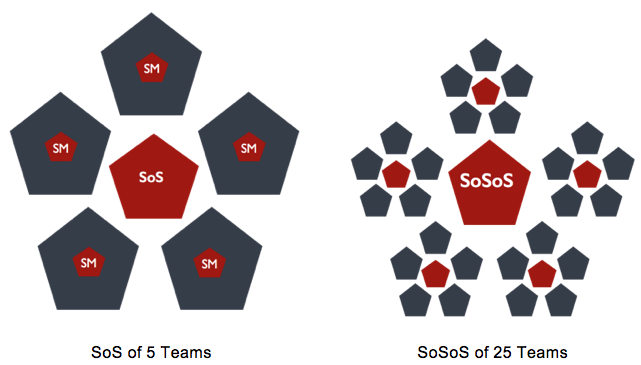
\includegraphics[width=1.0\linewidth]{Sos-R2.png}

\textbf{\textsc{nota:}} Ache se la Guida Scrum definisce la dimensione ottimale dell Team da 3 a 9 persone, ricerche di Harvard hanno determinato che la dimensione ottimale di una  squadra è di 4,6 persone\footnote{Hackman, J Richard, Leading teams: Setting the stage for
great performances, Harvard Business Press, 2002}. Esperimenti con Team altamente performanti hanno ripetutamente dimostrato che 4 o 5 persone coinvolte nel lavoro è la dimensione ottimale. È essenziale per la scalabilità lineare che questo modello sia lo stesso anche per il numero di Team in un SoS. Pertanto, nella figura sopra e nei diagrammi seguenti, sono stati scelti dei pentagoni per rappresentare una squadra di 5 persone. Questi diagrammi sono pensati per essere solo di esempio, i diagrammi reali di una organizzazione possono essere anche molto diversi.

\subsection{Lo Executive Action Team}
Lo Scrum of Scrums di una intera organizzazione è chiamato \textbf{Executive Action Team (EAT)}. The leadership team creates an agile bubble
in the organization where the reference model operates with 
its own guidelines and procedures that integrates effectively 
with any part of the organization that is not agile. It owns the agile ecosystem, 
implements the Scrum values, and assures that 
Scrum roles are created and supported.

The EAT is the final stop for
impediments that cannot be removed by the SoS's that feed it. Therefore, it
must be comprised of individuals who are empowered, politically and
financially, to remove them. 
The function of the EAT is to coordinate
multiple SoS's (or SoSoS's). As with any Scrum team, it needs a PO and SM.
It would be best if the EAT met daily as a Scrum team. They must meet at
least once per Sprint and have a transparent backlog.

%\pagebreak
Sample Diagram showing an EAT coordinating 5 groupings of 25 teams:

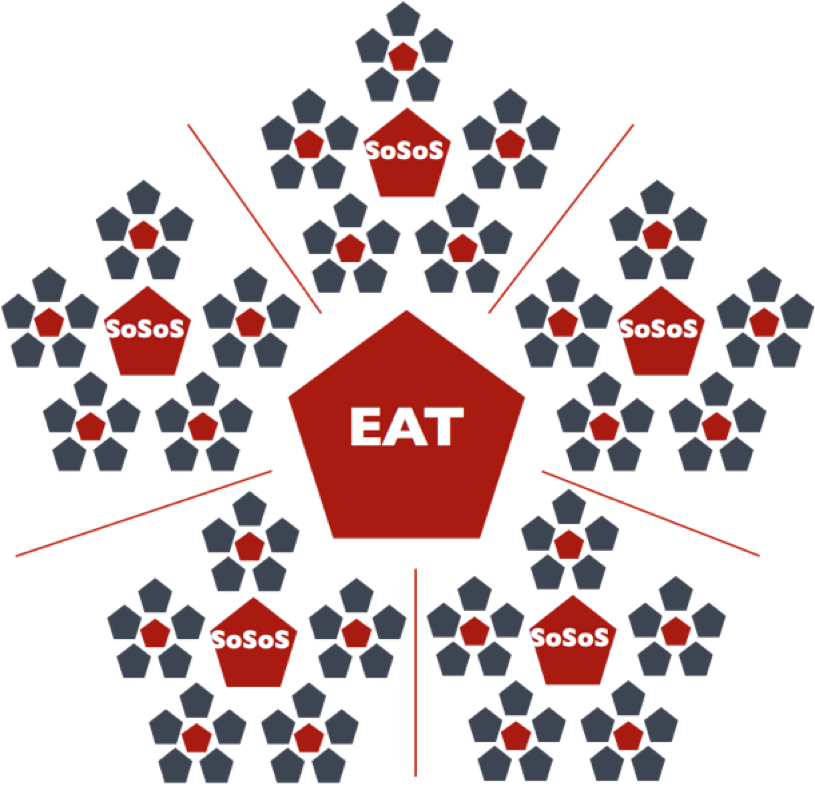
\includegraphics[width=\textwidth,height=\textheight,keepaspectratio]{SoS-EAT.png}

\subsection{The EAT's Backlog \& Responsibilities}
Scrum is an agile operating system that is different from traditional
project management. The entire SM organization reports into the EAT, which
is responsible for implementing this agile operating system by
establishing, maintaining, and enhancing the implementation in the
organization.
The EAT's role is to create an Organizational Transformation Backlog (a
prioritized list of the agile initiatives that need to be accomplished) and
see that it is carried out. For example, if there is a traditional Product
Development Life Cycle in the old organization, a new agile Product
Development Life Cycle needs to be created, implemented, and supported. It
will typically support quality and compliance issues better than the old
method but be implemented in a different way with different rules and
guidelines. The EAT ensures that a Product Owner organization is created and funded
and that this organization is represented on the EAT to support these efforts.

The EAT is accountable for the quality of Scrum within the organization.
Its responsibilities include but are not limited to:
\begin{itemize}
\item creating an agile operating system for the Reference Model as it
scales through the organization, including corporate operational rules,
procedures, and guidelines to enable agility.
\item measuring and improving the quality of Scrum in the organization.
\item building capability within the organization for business agility.
\item creating a center for continuous learning for Scrum professionals.
\item supporting the exploration of new ways of working.
\end{itemize}
Finally, the EAT must set up and support a corresponding Product Owner
organization through associations of PO's that mirror the SoS's and scale
their PO functions. These teams of PO's and key stakeholders are known as
\textbf{MetaScrums}.

\subsection{Outputs/Outcomes of the Scrum Master Cycle}
The SM organization (SoS, SoSoS, and EAT) work as a whole to complete the
other components of the Scrum Master Cycle: \textbf{Continuous Improvement
and Impediment Removal, Cross-Team Coordination, and Deployment}.

The goals of Continuous Improvement and Impediment Removal are to:
\begin{itemize}
\item identify impediments and reframe them as opportunities.
\item maintain a healthy and structured environment for prioritizing and
removing impediments, and then verifying the resulting improvements.
\item ensure visibility in the organization to effect change.
\end{itemize}
The goals of Cross-Team Coordination are to:
\begin{itemize}
\item coordinate similar processes across multiple related teams.
\item mitigate cross-team dependencies to ensure they don't become
impediments.
\item maintain alignment of team norms and guidelines for consistent output.
\end{itemize}

Since the goal of the SoS is to function as a release team, the deployment
of product falls under their scope, while what is contained in any release
falls under the scope of the Product Owners. Therefore, the goals of the
Deployment are to:
\begin{itemize}
\item deliver a consistent flow of valuable finished product to customers.
\item integrate the work of different teams into one seamless product.
\item ensure high quality of the customer experience.
\end{itemize}

\section{Product Owner Cycle}
\subsection{Coordinating the ``What'' - The MetaScrum}
A group of Product Owners who need to coordinate a single backlog that
feeds a network of teams are themselves a team called a \textbf{MetaScrum}.
For each SoS there is an associated MetaScrum. A MetaScrum aligns the
teams' priorities along a single path so that they can coordinate their
backlogs and build alignment with stakeholders to support the backlog.

MetaScrums hold a scaled version of Backlog Refinement, the \textbf{Scaled Backlog Refinement Meeting} 
\begin{itemize}
\item Each team PO (or proxy) must attend
\item This event is the forum for Leadership, Stakeholders, or other
Customers to express their preferences
\end{itemize}
This event occurs as often as needed, at least once per Sprint, to ensure a
Ready backlog. 

The main functions of the MetaScrum are to:
\begin{itemize}
\item create an overarching vision for the product \& make it visible to
the organization.
\item build alignment with key stakeholders to secure support for backlog
implementation.
\item generate a single, prioritized backlog; ensuring that duplication of
work is avoided.
\item create a uniform ``Definition of Done'' that applies to all teams in
the SoS.
\item eliminate dependencies raised by the SoS.
\item generate a coordinated Release Plan.
\item decide upon and monitor metrics that give insight into the product.
\end{itemize}
MetaScrums, just like SoS's, function as Scrum teams on their own. As such,
they need to have someone who acts as a SM and keeps the team on track in
discussions. They also need a single person who is responsible for coordinating the
generation of a single Product Backlog for all of the teams covered by the
MetaScrum. This person is designated as the \textbf{Chief Product Owner}.

\subsection{The Chief Product Owner (CPO)}
Through the MetaScrums, Chief Product Owners coordinate priorities among
Product Owners who work with individual teams. They align backlog
priorities with Stakeholder and Customer needs. Just like a SoSM, they may
be an individual team PO who chooses to play this role as well, or they may
be a person specifically dedicated to this role. Their main
responsibilities are the same as a regular PO's, but at scale:
\begin{itemize}
\item Setting a strategic vision for the whole product.
\item Creating a single, prioritized backlog of value to be delivered by
all of the teams.
\begin{itemize}
\item These items would be larger stories than that for a team PO.
\end{itemize}
\item Working closely with their associated SoSM so that the Release Plan
that the MetaScrum team generates can be deployed efficiently.
\item Monitoring customer product feedback and adjusting the backlog
accordingly.
\end{itemize}

\subsection{Scaling the MetaScrum}
Just as SoS's can grow into SoSoS's, MetaScrums can also expand by the same
mechanism. There is no specific term associated with these expanded units,
nor do the CPO's of them have specific expanded titles. We encourage each
organization to develop their own. For the following diagrams, we have
chosen to add an additional ``Chief'' to the title of those PO's as they
magnify out.

%\pagebreak
Some sample diagrams:

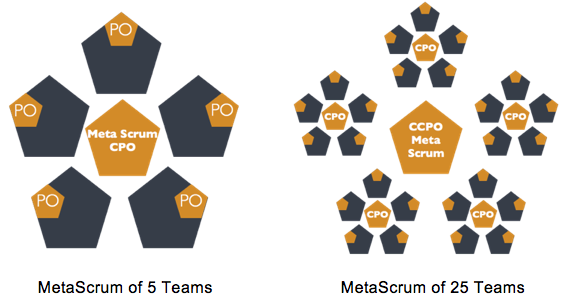
\includegraphics[width=1.0\linewidth]{MetaScrum-R2.png}

\textbf{NOTE:} As mentioned above, these pentagons represent the ideal
sized Scrum teams and ideal sized MetaScrums. These diagrams are meant to
be examples only, your organizational diagram may differ greatly.

\subsection{The Executive MetaScrum (EMS)}
The MetaScrums enable a network design of Product Owners which is
infinitely scalable alongside their associated SoS's. The MetaScrum for the
entire agile organization is the \textbf{Executive MetaScrum}. The EMS owns
the organizational vision and sets the strategic priorities for the whole
company, aligning all the teams around common goals.

Sample diagram showing an EMS coordinating 5 groups of 25 teams:

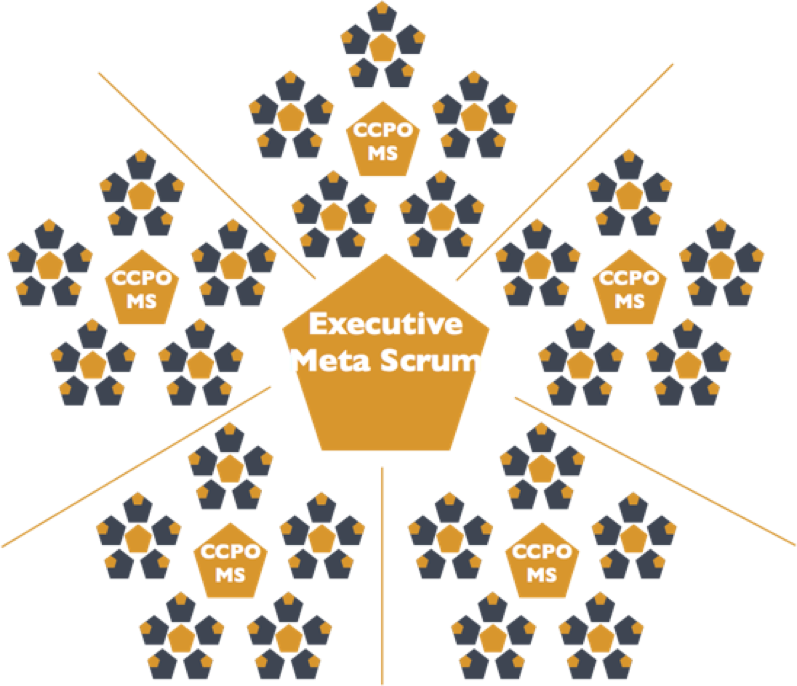
\includegraphics[width=1.0\linewidth]{ExecMetaScrum.png}

\subsection{Outputs/Outcomes of the Product Owner Organization}
The PO organization (various MetaScrums, the CPO's, and the Executive
MetaScrum) work as a whole to satisfy the components of the Product Owner
Cycle: \textbf{Strategic Vision, Backlog Prioritization, Backlog
Decomposition \& Refinement, and Release Planning}.

The goals of setting a Strategic Vision are to:
\begin{itemize}
\item clearly align the entire organization along a shared path forward.
\item compellingly articulate why the organization exists.
\item describe what the organization will do to leverage key assets in
support of its mission.
\item respond to rapidly changing market conditions.
\end{itemize}
The goals of Backlog Prioritization are to:
\begin{itemize}
\item identify a clear ordering for products, features, and services to be
delivered.
\item reflect value creation, risk mitigation and internal dependencies in
ordering of the backlog.
\item prioritize the high-level initiatives across the entire agile
organization prior to Backlog Decomposition and Refinement.
\end{itemize}
The goals of Backlog Decomposition \& Refinement are to:
\begin{itemize}
\item break complex products and projects into independent functional
elements that can be completed by one team in one Sprint.
\item capture and distill emerging requirements and customer feedback.
\item ensure all backlog items are truly ``Ready'' so that they can be
pulled by the individual teams.
\end{itemize}
The goals of Release Planning are to:
\begin{itemize}
\item forecast delivery of key features and capabilities.
\item communicate delivery expectations to stakeholders.
\item update prioritization, as needed.
\end{itemize}

\section{Connecting the PO/SM Cycles}

\subsection{Understanding Feedback}
The \textbf{Feedback} component is the second point where the PO \& SM
Cycles touch. Product feedback drives continuous improvement through
adjusting the Product Backlog while Release feedback drives continuous
improvement through adjusting the Deployment mechanisms. The goals of
obtaining and analyzing Feedback are to:
\begin{itemize}
\item validate our assumptions.
\item understand how customers use and interact with the product.
\item capture ideas for new features and functionality.
\item define improvements to existing functionality.
\item update progress towards product/project completion to refine release
planning and stakeholder alignment.
\item identify improvements to deployment methods and mechanisms.
\end{itemize}

\subsection{Metrics \& Transparency}
Radical transparency is essential for Scrum to function optimally, but it
is only possible in an organization that has embraced the Scrum values. It
gives the organization the ability to honestly assess its progress and to
inspect and adapt its products and processes. This is the foundation of the
empirical nature of Scrum as laid out in the Scrum Guide.

Both the SM \& PO Cycles require metrics that will be decided upon by the
separate SM and PO organizations. Metrics may be unique to both specific
organizations as well as to specific functions within those organizations.
Scrum@Scale does not require any specific set of metrics, but it does
suggest that at a bare minimum, the organization should measure:
\begin{itemize}
\item Productivity - e.g. change in amount of Working Product delivered per
Sprint
\item Value Delivery - e.g. business value per unit of team effort
\item Quality - e.g. defect rate or service downtime
\item Sustainability - e.g. team happiness
\end{itemize}
The goals of having Metrics and Transparency are to:
\begin{itemize}
  \item provide all decision makers, including team members, with
appropriate context to make good decisions.
\item shorten feedback cycles as much as possible to avoid over-correction.
\item require minimal additional effort by teams, stakeholders or
leadership.
 \end{itemize}

\subsection{Some notes on Organizational Design}
The scale-free nature of Scrum@Scale allows the design of the organization
to be component-based, just like the framework itself. This permits for
rebalancing or refactoring of teams in response to the market. As an
organization grows, capturing the benefits of distributed teams may be
important. Some organizations reach talent otherwise unavailable and are
able to expand and contract as needed through outsourced development.
Scrum@Scale shows how to do this while avoiding long lag times, compromised
communications, and inferior quality, enabling linear scalability both in
size and global distribution.\footnote{Sutherland, Jeff and Schoonheim,
Guido and Rustenburg, Eelco and Rijk, Maurits, ``Fully distributed scrum:
The secret sauce for hyperproductive offshored development teams'',
AGILE'08. Conference, IEEE: 339-344, 2008}

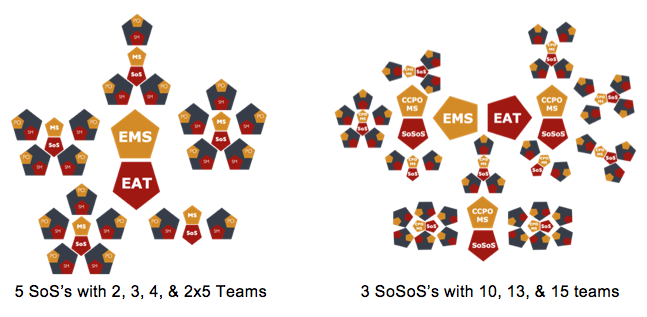
\includegraphics[width=1.0\linewidth]{VariableSoS-R2.png}
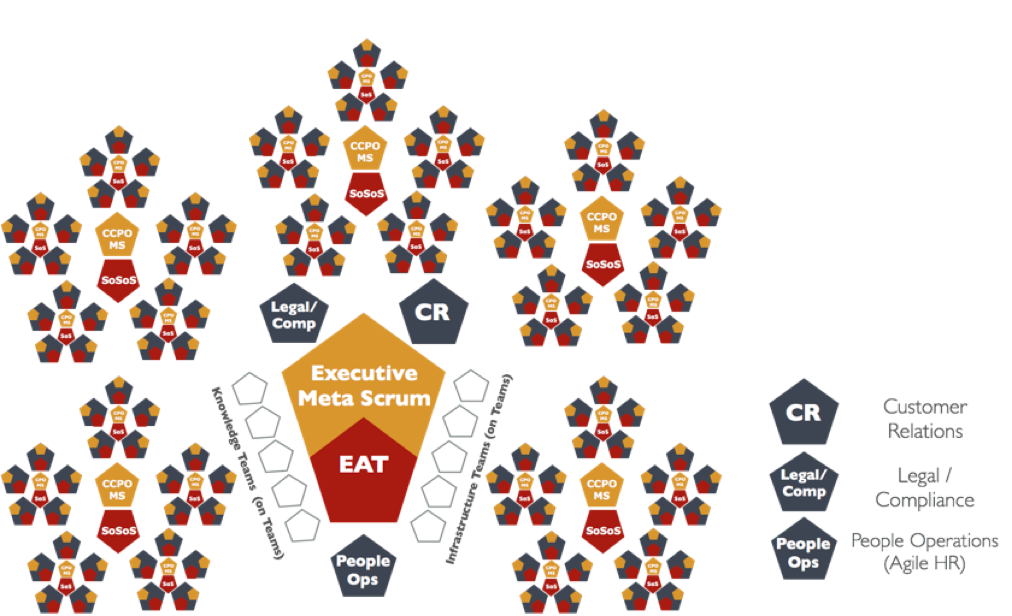
\includegraphics[width=1.0\linewidth]{OrganizationalDiagram.png}

In this organizational diagram, the \textbf{Knowledge \& Infrastructure
Teams} represent virtual teams of specialists of which there are too few to
staff each team. They coordinate with the Scrum teams as a group via
service-level agreements where requests flow through a PO for each
specialty who converts them into a transparent ordered backlog. An
important note is that these teams are NOT silos of individuals who sit
together (this is why they are represented as hollow pentagons); their team
members sit on the actual Scrum teams, but they make up this virtual Scrum
of their own for the purpose of backlog dissemination and process
improvement.

\textbf{Customer Relations, Legal / Compliance, and People Operations} are
included here since they are necessary parts of organizations and will
exist as independent Scrum teams on their own, which all of the others may
rely upon.

A final note on the representation of the EAT \& EMS: in this diagram, they
are shown as overlapping since some members sit on both of the teams. In very
small organizations or implementations, the EAT \& EMS may consist entirely
of the same team members.

\section{End Note}
Scrum@Scale is designed to scale productivity, to get the entire
organization doing twice the work in half the time with higher quality and
in a significantly improved work environment. Large organizations that
properly implement the framework can cut the cost of their products and
services while improving quality and innovation.

Scrum@Scale is designed to saturate an organization with Scrum. All teams,
including Leadership, Human Resources, Legal, Consulting \& Training, and
product \& service teams, implement the same style of Scrum while
streamlining and enhancing an organization.

Well implemented Scrum can run an entire organization.

\section{Acknowledgements}
We acknowledge IDX for the creation of the Scrum of Scrums which first
allowed Scrum to scale to hundreds of teams,\footnote{Sutherland, Jeff,
``Inventing and Reinventing SCRUM in five Companies'', Sur le site officiel
de l'alliance agile, 2001} PatientKeeper for the creation of the
MetaScrum,\footnote{Sutherland, Jeff, ``Future of scrum: Parallel pipelining
of sprints in complex projects'', Proceedings of the Agile Development
Conference,  IEEE Computer Society 90-102,  2005.} which enabled rapid
deployment of innovative product, and OpenView Venture Partners for scaling
Scrum to the entire organization.\footnote{Sutherland, Jeff and Altman,
Igor, ``Take no prisoners: How a venture capital group does scrum'', Agile
Conference, 2009. AGILE'09, IEEE 350-355.  2009} We value input from Intel
with over 25,000 people doing Scrum who taught us ``nothing scales'' except
a scale-free architecture, and SAP with the largest Scrum team product
organization who taught us management involvement in the MetaScrum is
essential to get 2,000 Scrum teams to work together.

The agile coaches and trainers implementing these concepts at Amazon, GE,
3M, Toyota, Spotify, Maersk, Comcast, AT\&T and many other companies working with Jeff Sutherland
have been helpful in testing these concepts across a wide range of
companies in different domains.

And finally, Avi Schneier and Alex Sutherland have been invaluable in
formulating and editing this document.

\pagebreak

\printbibliography



\end{document}
